\chapter{Discretization of the Grad-Shavranov equation}\label{chapter:sem}
In this chapter in first place we set the Grad-Shavranov equation, cmp. Sec.(\ref{sec:grad_shavranov}), in an appropriate domain and, starting from the physic of the problem, we choose reasonable boundary conditions which respect the physic. After that, we rigorously compute the variational formulation of the problem since we are going to solve it with a Galerkin method. Finally we shortly explain the spectral element method and we calculate the discretized expression of our problem.

\section{The Equilibrium problem for fixed conditions}\label{sec:eq_problem_fixed_bc}
We want to solve numerically the equilibrium equation (\ref{eq:GS_eq}), derived in Sec.(\ref{sec:grad_shavranov}), that we report for simplicity
\begin{equation}\label{eq:compact_equlibrium}
  -\Delta^*\psi(r,z)=-\mathbf{F}(r,z,B,\psi,\nabla B, \nabla\psi)\cdot\nabla\psi(r,z)+r^2\:f(r,z,B,\psi)
\end{equation}
in the domain $\Omega$, where
\begin{equation}\label{eq:functional_F}
  \mathbf{F}(r,z,B,\psi,\nabla B, \nabla\psi)=\frac{1}{1-\frac{\partial_B p_\parallel(\psi,B)}{B(r,z,|\nabla\psi|)}}\nabla \Big(\frac{\partial_B p_\parallel(\psi,B)}{B(r,z)}\Big)
\end{equation}
and
\begin{equation}
  f(r,z,B,\psi)=\frac{1}{1-\frac{\partial_B p_\parallel(\psi,B)}{B(r,z,|\nabla\psi|)}}\partial_\psi p_\parallel(\psi,B),
\end{equation}
using fixed boundary condition. Therefore our domain is not the geometrical surface enclosed by the mirror machine but it is the inner region occupied exclusively by plasma.
\medskip

In Fig.(\ref{fig:mirror_domain}) we show the domain $\Omega$ where we are going to solve the problem. The horizontal axis corresponds to the symmetry axis $z$ while the vertical one corresponds to the cylindrical coordinate $r$. We have normalized all the quantities respect to the horizontal length $L$ of the domain, which has been imposed unitary, so $L=1$, and $0\leq z\leq 1$.

Since we have a longitudinally directed magnetic field, we look for solutions satisfying periodic boundary condition in $z$-direction \cite[\S 6.2]{magnetic_mirror} and we have $\frac{\partial\mathbf{B}}{\partial r}|_{\Gamma_1}=0$. To impose this periodicity, the border $\Gamma_1$ have to intersect $\Gamma_2$ and $\Gamma_4$ perpendicularly. We choose for $\Gamma_1$ a sinusoidal shape because it is close to the shape of the magnetic field; more precisely we use
\begin{equation}\label{eq:border_equation}
  \gamma:r=\frac{1}{25}\sin(2\pi(z-\frac{1}{4}))+\frac{1}{5}.
\end{equation}

\begin{figure}
\centering
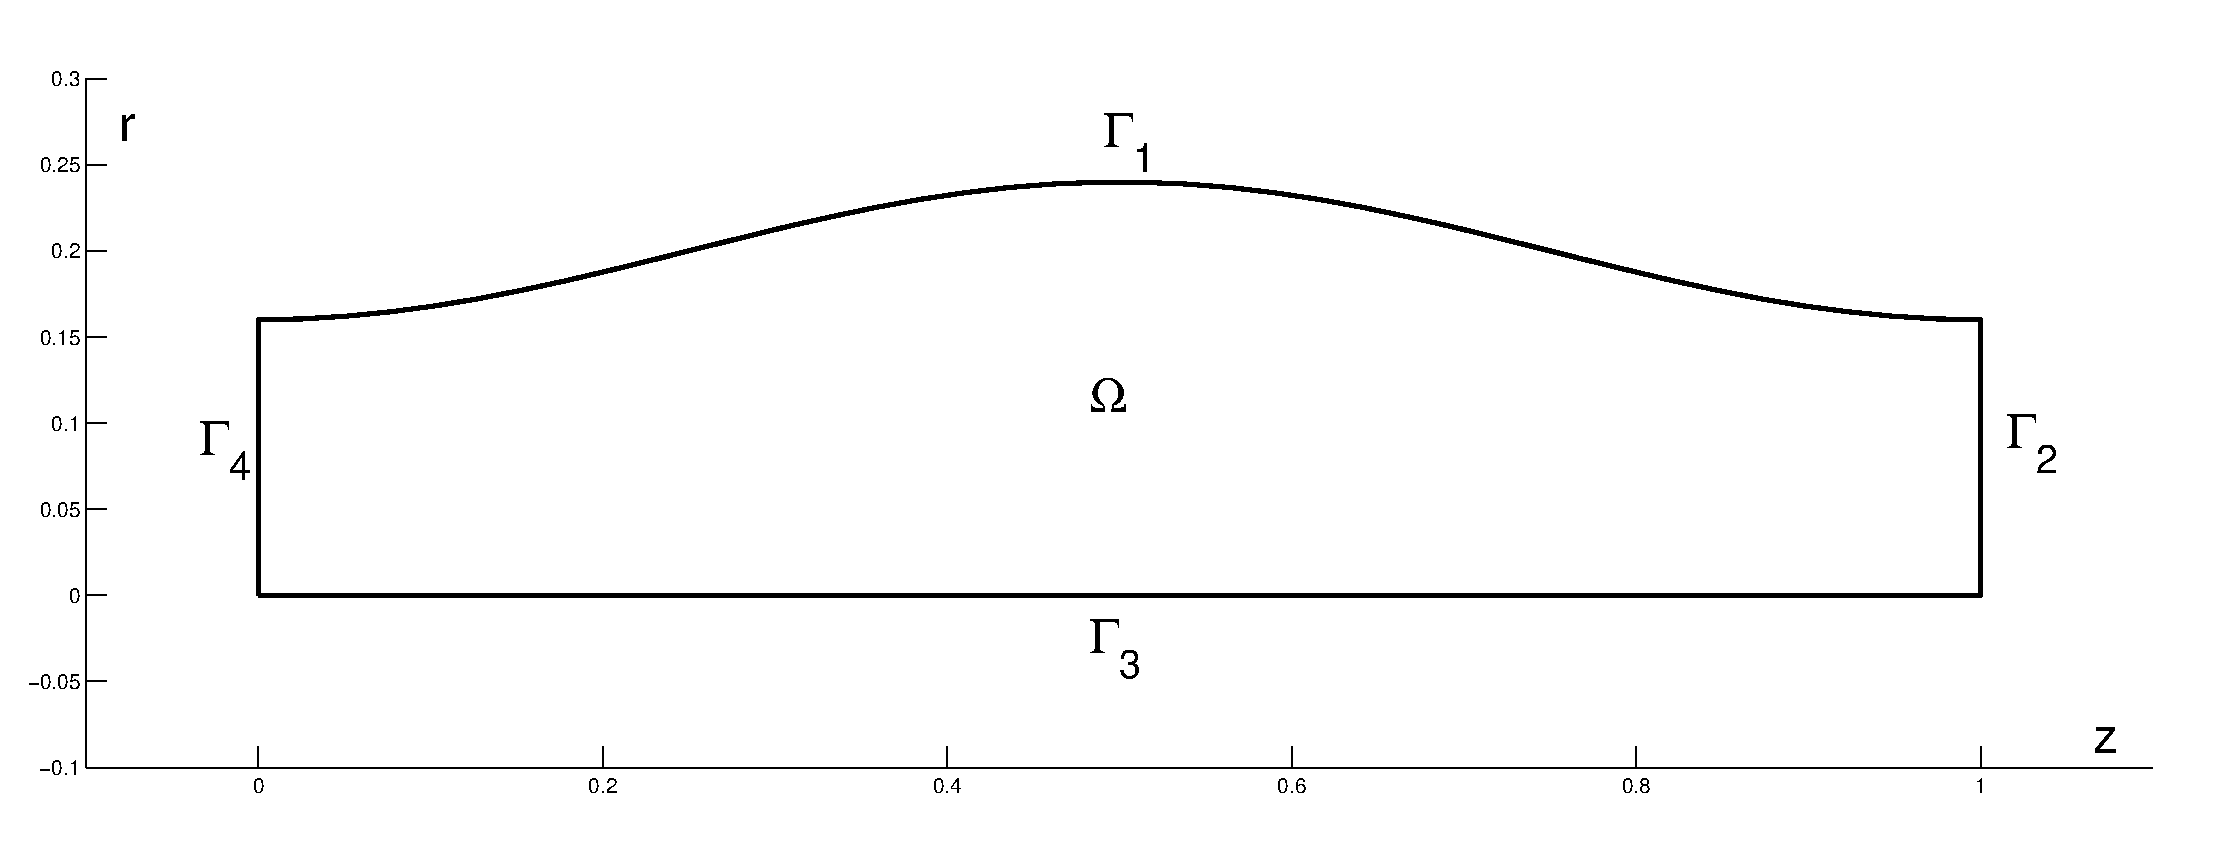
\includegraphics[scale=0.4]{images/mirror_matlab.eps}
\caption{Computational domain $\Omega$ for the fixed-boundary problem.}\label{fig:mirror_domain}
\end{figure}

From the physics of the problem, it makes sense to impose the following boundary conditions:
\begin{itemize}
  \item On $\Gamma_1$ Dirichlet;
  \item On $\Gamma_2$ periodicity with $\Gamma_4$
\end{itemize}
which are equivalent to
\begin{equation}\label{eq:bc}
  \begin{cases}
    \psi|_{\Gamma_1}=g(z)\\
    \psi|_{\Gamma_2}=\psi|_{\Gamma_4}\\
    \nabla\psi|_{\Gamma_2}=\nabla\psi|_{\Gamma_4}.
  \end{cases}
\end{equation}

It is important to notice that no condition are imposed on the boundary $\Gamma_3$. This happens since we are using the axisymmetric hypothesis therefore no condition can be imposed there. In the following section, cmp. Sec.(\ref{sec:weak_formulation}), this fact will come out naturally from the weak formulation.

Therefore the equilibrium problem is the following:
\begin{equation}\label{eq:equlibrium_and_bc}
  \begin{cases}
    -\Delta^*\psi+\mathbf{F}\cdot\nabla\psi-r^2\:f=0 & \mathrm{in}\:\Omega\\
    \psi(z,\gamma(z))=g(z)& \\
    \psi(0,r)=\psi(1,r)\\
    \nabla\psi(0,r)=\nabla\psi(1,r).
  \end{cases}
\end{equation}

\section{Weak formulation}\label{sec:weak_formulation}
For the numerical discretization we need to derive the weak form, or distributional formulation, of Eq.(\ref{eq:compact_equlibrium}), which requires less regularity on the solution, at the expense of increasing the regularity requirement on the test functions.
\medskip

The Laplace operator in cylindrical coordinates, under axisymmetric hypothesis, assumes the following expression
\begin{equation}\label{eq:laplace_operator}
  \Delta f=\frac{1}{r}\frac{\partial}{\partial r}\bigg(r\frac{\partial f}{\partial r}\bigg)+\frac{\partial^2f}{\partial z^2}=\frac{\partial^2f}{\partial r^2}+\frac{\partial^2f}{\partial z^2}+\frac{1}{r}\frac{\partial f}{\partial r},
\end{equation}
while the gradient has the same expression
\begin{equation}\label{eq:gradient_operator}
  \nabla f=\frac{\partial f}{\partial r}\mathbf{e}_r+\frac{\partial f}{\partial z}\mathbf{e}_z,
\end{equation}
therefore the Grad-Shafranov operator, cmp. Eq.(\ref{eq:GS_operator}), defined as
\begin{equation}
  \Delta^* \psi=\Delta\psi-\frac{2}{r}\partial_r\psi;
\end{equation}
assumes the following formulation
\begin{equation}\label{eq:GS_explicit}
  \Delta^* \psi=\partial_{rr}\psi+\partial_{zz}\psi-\frac{1}{r}\partial_r\psi.
\end{equation}
We can rewrite Eq.(\ref{eq:compact_equlibrium}), substituting inside Eq.(\ref{eq:GS_explicit}) and multiplying  everything by $r$ to get rid of the denominator, as
\begin{equation}\label{eq:compact_equlibrium_bis}
  -r\:(\partial_{rr}\psi+\partial_{zz}\psi)+\partial_r\psi+r\:\mathbf{F}\cdot\nabla\psi-r^3\:f=0
\end{equation}
which in ,distributional formulation, becomes
\begin{equation}\label{eq:compact_equlibrium_var}
  -\int_{\Omega}(\partial_{rr}\psi+\partial_{zz}\psi)\:rv\:\mathrm{d}\Omega + \int_{\Omega}\partial_r\psi\:v\:\mathrm{d}\Omega + \int_{\Omega}\mathbf{F}\cdot\nabla\psi\:rv\:\mathrm{d}\Omega - \int_{\Omega}r^3\:f\:v\:\mathrm{d}\Omega = 0.
\end{equation}
Applying the divergence theorem to the first term
\begin{equation}\label{eq:divergence_theorem}
  -\int_V (\partial_{rr}u+\partial_{zz}u)\:w\:\mathrm{d}V= \int_V \nabla u\cdot\nabla w\mathrm\:{d}V-\int_S w\nabla u\cdot\mathrm{d}\mathbf{S},
\end{equation}
taking $w=rv$ and $u=\psi$ over the domain $\Omega$, we obtain
\begin{equation}\label{eq:weak_GS_second_order_term}
  -\int_{\Omega}(\partial_{rr}u+\partial_{zz}u)\:rv\:\mathrm{d}\Omega=\int_\Omega \nabla\psi \cdot\nabla(rv)\:\mathrm{d}\Omega -\int_{\partial\Omega} rv\nabla \psi\cdot\mathrm{d}\mathbf{\partial\Omega}.
\end{equation}
The volume integral of Eq.(\ref{eq:weak_GS_second_order_term}), using the fact that
\begin{equation}
  \nabla(rv)=r\nabla v+v\left(\begin{array}{c}0\\1\end{array}\right),
\end{equation}
can be rewritten as
\begin{equation}
  \int_\Omega\nabla\psi \cdot\nabla(rv)\:\mathrm{d}\Omega=\int_\Omega r\:\nabla\psi \cdot\nabla v\:\mathrm{d}\Omega+\int_{\Omega}\partial_r\psi\:v\:\mathrm{d}\Omega
\end{equation}
while the surface integral becomes
\begin{equation}
  -\int_{\partial\Omega} rv\nabla \psi\cdot\mathrm{d}\mathbf{\partial\mathbf{\Omega}} = -\int_{\Gamma_1} rv\nabla \psi\cdot\mathrm{d}\mathbf{\Gamma}_1 - \int_0^{\gamma(1)}r(v\:\partial_z\psi)|_{z=1}\:\mathrm{d}r + \int_0^{\gamma(0)}r(v\:\partial_z\psi)|_{z=0}\:\mathrm{d}r
\end{equation}
where the line integral over $\Gamma_3$ is null due to the fact that $r=0$. Moreover it holds
\begin{equation}
  \begin{split}
    -\int_0^{\gamma(1)}r(v\:\partial_z\psi)|_{z=1}\:\mathrm{d}r + \int_0^{\gamma(0)}r(v\:\partial_z\psi)|_{z=0}\:\mathrm{d}r=\\
  =\int_0^{\gamma(1)=\gamma(0)}r\big((v\:\partial_z\psi)|_{z=0}-(v\:\partial_z\psi)|_{z=1}\big)\mathrm{d}r;
  \end{split}
\end{equation}
the quantity $(v\:\partial_z\psi)|_{z=0}-(v\:\partial_z\psi)|_{z=1}$ is the jump of the function $\partial_z\psi \:v$ on the line where we impose the periodicity, therefore $\Gamma_2\equiv\Gamma_4$. From the periodicity conditions, cmp. Eq.(\ref{eq:equlibrium_and_bc}), we know that $\psi\in C^1(\Gamma_2\equiv\Gamma_4)$ and $v\in C^0(\Gamma_2\equiv\Gamma_4)$ therefore $\partial_z\psi\:v\in C^0(\Gamma_2\equiv\Gamma_4)$ and its jump on that line must be equal to zero which leads to
\begin{equation}
  \int_0^{\gamma(1)=\gamma(0)}r\big((v\:\partial_z\psi)|_{z=0}-(v\:\partial_z\psi)|_{z=1}\big)\mathrm{d}r=0.
\end{equation}
Therefore we can rewrite Eq.(\ref{eq:weak_GS_second_order_term}) as
\begin{equation}
  -\int_{\Omega}(\partial_{rr}u+\partial_{zz}u)\:rv\:\mathrm{d}\Omega=\int_\Omega r\:\nabla\psi \cdot\nabla v\:\mathrm{d}\Omega+\int_{\Omega}\partial_r\psi\:v\:\mathrm{d}\Omega-\int_{\Gamma_1} rv\nabla \psi\cdot\mathrm{d}\mathbf{\Gamma}_1
\end{equation}
which leads to the the following weak formulation for Eq.(\ref{eq:equlibrium_and_bc})
\begin{equation}\label{eq:GS_BC_weak}
  \begin{split}
    \int_\Omega r\:\nabla\psi \cdot\nabla v\:\mathrm{d}\Omega+2\int_\Omega v\:\partial_r \psi\:\mathrm{d}\Omega+\int_\Omega rv\:\mathbf{F}(\psi,B)\cdot\nabla\psi\:\mathrm{d}\Omega +\\ -\int_\Omega r^3vf\:\mathrm{d}\Omega =\int_{\Gamma_1} rv\nabla \psi\cdot\mathrm{d}\mathbf{\Gamma}_1\quad\forall v\in V.
  \end{split}
\end{equation}
\medskip

In order to define the space of solution and test functions, the integrals in Eq.(\ref{eq:GS_BC_weak}) must have sense, which means that integrands must be in $L^1(\Omega)$. To satisfy this condition we use the H\"{o}lder's inequality in his generalized version: assume that $p\in(0, \infty)$ and $p_1,\dots, p_n  \in (0, \infty]$ such that
\begin{equation}
  \sum_{k=1}^n \frac1{p_k}=\frac{1}{p}
\end{equation}
than
\begin{equation}
  f_k\in L^{p_k}(\mu)\;\;\forall k\in\{1,\ldots,n\}\implies\prod_{k=1}^n f_k \in L^p(\mu).
\end{equation}
Since $r\in L^\infty(0,R)$ and also its positive integer powers, then we required at least that $\nabla \psi$, $\psi$ and $\nabla v$, $v$ are in $L^2(\Omega)$,
i.e.$\psi,v\in H^1(\Omega)$. In addition we need the nonlinear terms be $\mathbf{F}\in L^\infty(\Omega)$ and $f\in L^2(\Omega)$. These last assumptions are not trivial.
\medskip

We want to use a Galerkin formulation therefore we need to define the test space and the trial space as close as possible. Usually the space where we look for the solution is influenced by the Dirichlet conditions, in particular that ones in (\ref{eq:bc}) can be included fully in the trial space, instead the test functions can vanish on the Dirichlet boundary. Let the test space be
\begin{equation}\label{eq:test_space}
\begin{split}
 V&=\{v\in H^1(\Omega):\:v|_{\Gamma_1}=0\}\cap\{v\in H^1(\Omega):\:v|_{\Gamma_3}=0 \}\\
&\cap\{v\in C^0(\overline{\Omega}):v|_{\Gamma_2}=v|_{\Gamma_4}\}=V_0^{\Gamma_1}\cap V_0^{\Gamma_3} \cap C^0(\Omega)=V_0 \cap C^0(\Omega)
\end{split}
\end{equation}
and let the trial space be
\begin{equation}\label{eq:trial_space}
 W=V_0^{\Gamma_3}\cap\{v\in H^1(\Omega):\:v|_{\Gamma_1}=g \}\cap C^0_{p_z}(\Omega)=V_0^{\Gamma_3}\cap V_g^{\Gamma_1}\cap C^0(\Omega).
\end{equation}

$V_g$ is an affine manifold of $H^1(\Omega)$, not a subspace of $H^1(\Omega)$ therefore it is not possible to express the solution as an expansion of a basis as it is not true that linear combinations of elements in $V_g$ are still elements of $V_g$. There are two usual ways to treat this problem:
\begin{itemize}
  \item if $g\in H^{1/2}(\Gamma_1)$, so $\exists\: R_g\in H^1(\Omega)$, called Dirichlet lift, such that $R_g|_{\Gamma_1}=g$, the solution can be split into two contributions $\psi=\psi_0+R_g$, where $\psi_0\in V$ and $R_g\in V_g$;
  \item the matrix system can be assembled including all degrees of freedom of our approximation and then we can zeroing the rows which correspond to the Dirichlet degree of freedom,
  placing a unit term on the diagonal and setting the right-hand side to the known values. It means that we look for $\psi\in V_0^{\Gamma_3}\cap C^0(\Omega)$ such that $\psi|_{\Gamma_1}=g$.
\end{itemize}
Numeric approximation makes easy the task of building the Dirichlet lift: it can be done from an approximation of the boundary data $g$, generally as a linear combination of the basis function on the Dirichlet boundaries. This splitting technique is useless when we have to treat nonlinear term and we can only apply the zeroing technique at the final system. So we look for the complete solution though the knowledge of the value of the solution on the Dirichlet boundaries making its calculations useless and the final problem will not be yet symmetric since we request, in principle, different constraints to the trial and test spaces.

In the light of space definitions, the weak formulation (\ref{eq:GS_BC_weak}) becomes
\begin{equation}\label{eq:prob_var}
  \left\{\begin{array}{ll}\textrm{Find $\psi\in W$ such that}\\
  \textrm{$a(\psi,v)=0$ $\forall v\in V$ and $\psi|_{\Gamma_3}=g$}\\
\end{array}\right.
\end{equation}
where $a(\psi,v)$ is the nonlinear map $a:W_g\times V_0\rightarrow\mathbb{R}$:
\begin{equation}\label{eq:a_operator}
  a(\psi,v)=\int_\Omega \big(r\:\nabla\psi \cdot\nabla v+2v\:\partial_r \psi+rv\:\mathbf{F}\cdot\nabla\psi -r^3vf\big)\mathrm{d}\Omega.
\end{equation}
Since the mapping is nonlinear $a(u_0+R_g,v)\neq a(u_0,v)+a(R_g,v)$ which implies that it is not possible to use the Dirichlet lift to impose Dirichlet boundary conditions but it is necessary to apply the zeroing technique.

\section{Spectral element method}\label{sec:spectral_aproximation}
Spectral Element Method (SEM) is a particular type of Finite Element Method (FEM). The difference with a classical FEM are the interpolation nodes, indeed for the former they are distributed at position corresponding to the zeros of a family of orthogonal polynomials while for the latter on some special points on the element.

The choice of an orthogonal basis allows the accuracy of the method to be spectral, i.e. the rate of convergence of the interpolation with respect to degree $p=\min p_m$ of polynomial is faster than any power of $1/p$. Indeed its order of convergence is related to the maximum regularity of the solution, namely it is exponential for a very smooth solution but this fast convergence is easily lost if the solution has finite regularity or if the domain is irregular. In this case the order of convergence is reduced to a classical FEM where it is fixed by the choice of the basis and it does not depend on the regularity of the solution.

Unfortunately the stiffness matrix which arise from a SEM discretization is more dense than the one generated by a classical FEM, therefore the computational cost is higher. For this reason it is worthing to use this type of discretization when a smooth solution is expected, which it is our case since we are solving an equilibrium problem.

In the following we give a brief overview of the method and we point out the concepts which will be important in the implementation of the code. For an introductory description cmp. \cite{QUARTERONI} while for a more advance analysis  of the method cmp. \cite{CHQZ06} for 1-D domains and \cite{CHQZ07} for multidimensional domains. For what concern the implementation cmp. \cite{KARNIADAKIS} and \cite{HENDERSON}.

\subsection{Spectral element}\label{subsec:sem_element}
The mirror domain $\Omega\subset\mathbb{R}^2$, see Fig.(\ref{fig:mirror_domain}), can be represented as a union of $M$ disjoint quadrilateral sub-domain $\Omega_m$ with straight edges:
\begin{equation}
  \Omega\approx\mathcal{T}_h=\bigcup_{m=1}^M\Omega_m.
\end{equation}
We consider only a geometrically conforming partition which means that neighboring sub-domains share either a vertex or a complete edge. Let $h$ be
\begin{equation}
  h=\max_m h_m=\max_m\big(\mathrm{diam}(\Omega_m)\big)
\end{equation}
where $\mathrm{diam}(\Omega_m)$ is the length of longest edge of the element $\Omega_m$. Moreover we assume that these diameters are uniformly bounded below.

We define \textit{spectral element} the triplet $(\Omega_m, \mathbb{Q}_{p_m}(\Omega_m),\{v_k\})$ where
\begin{itemize}
  \item $\Omega_m$ convex quadrilateral $\subset \Omega$ so that $\Omega_m=\textbf{F}_m(\hat{\Omega})$;
  \item $\mathbb{Q}_{p_m}(\Omega_m)$ space of polynomials of degree $\leq p_m$ in each coordinate in $\Omega_m$, which dimension is $N=(p_m+1)^2$
  \item $\{v_k\}_0^N$ degrees of freedom for $\mathbb{Q}_{p_m}(\Omega_m)$
\end{itemize}

To standardize the local basis on $\Omega_m$, we introduce a logical domain $\hat{\Omega}=[-1,1]\times[-1,1]$ and an invertible bilinear map $\textbf{F}_m$,
\begin{equation}
\textbf{F}_m:\hat{\Omega} \rightarrow \Omega_m,
\end{equation}
between these two spaces. The maps which we will use it is not affine therefore it does not preserve the parallel property of edges and faces therefore the partition of the domain, in general, is not made by parallelogram. The explicit equation of the map used is given in Sec.(\ref{subsec:mapping}).
\medskip

We want to approximate our problem projecting it onto a space of functions that are piecewise polynomials on the element $\Omega_m$. We define the family of finite spaces of trial functions $W_\delta\subset W\subset C^0(\Omega)$
\begin{equation}
  W_\delta=\{w\in W:\: w|_{\Omega_m}=\hat{v}\circ \mathbf{F}^{-1}_m,\:\hat{v}\in\mathbb{Q}_{p_m}(\hat{\Omega})\:\forall\Omega_m\in\mathcal{T}_h\}
\end{equation}
and, analogously, the finite trial space is
\begin{equation}
 V_\delta=\{v\in V:\: v|_{\Omega_m}=\hat{v}\circ \mathbf{F}^{-1}_m,\:\hat{v}\in\mathbb{Q}_{p_m}(\hat{\Omega})\:\forall\Omega_m\in\mathcal{T}_h\}.
\end{equation}
where the subindex $\delta$ is an abridged notation for \textquotedblleft{discrete\textquotedblright} that accounts for the geometric sizes $h$ and the polynomial degrees $p=\min_m(p_m)$.

Ergo these two spaces are formed by functions that are images of polynomial functions $\hat{v}\in\mathbb{Q}_{p_m}(\Omega_m)$ through $\mathbf{F}_m$, so $v(x,y)=\hat{v}(\mathbf{F}_m^{-1}(x,y))$ $\forall(x,y)\in\Omega_m$. It is important to notice that $\mathbf{F}_m$ describes only the geometric transformation, whereas the function $v$ is not more a polynomial of the same degree of $\hat{v}$ as $\mathbf{F}_m$ is not affine.

In general both the mapping $\mathbf{F}_m$ and the polynomial order $p_m$  can vary within each element $\Omega_m$ thereby permitting both $h$- type refinement which alters $\mathbf{F}_m$ and $M$, and $p$-type refinement witch alters $p_m$. It is for this reason that SEM is called also $hp$-FEM. The polynomial basis chosen is given in Sec.(\ref{sec:modal_basis}).

\subsection{SEM}
The \textit{Galerkin approximation} consists in substitute the exact solution $\psi$ with the approximate solution $\psi_{\delta}$ into the weak formulation of our problem, cmp. Eq.(\ref{eq:prob_var}),
\begin{equation}
 \psi_\delta\in W_\delta:\: a(\psi_\delta,v_\delta)=0\quad\forall v_\delta\in V_\delta
\end{equation}
or, exploiting the linearity of the integral operator $a_m(u,v)=a(u,v)|_{\Omega_m}$,
\begin{equation}\label{eq:sem_formulation}
 \psi_\delta\in W_\delta:\: \sum_{m=1}^M a_m(\psi_\delta,v_\delta)=0\quad\forall v_\delta\in V_\delta
\end{equation}
which is the SEM formulation of our original problem.
\medskip

The discrete solution $\psi_{\delta}$ can be written as the truncated series on the global basis $\{\phi_k\}\in W_{\delta}$ or in the local one $\{\phi_j^{(m)}\}\in\mathbb{Q}_{p_m}(\Omega_m)$ in the following way
\begin{equation}\label{eq:solution_series}
  \psi_\delta=\sum_k \psi_k \phi_k=\sum_{m=1}^{M} \sum_{j=0}^{p^2_m} \psi^{(m)}_j \phi_j^{(m)}.
\end{equation}
Taking the scalar product of Eq.(\ref{eq:solution_series}) with $\phi_i$
\begin{equation}
  (\psi_\delta,\phi_i)=\sum_k \psi_k (\phi_k,\phi_i)
\end{equation}
we obtain the definition of the coefficients of the expansion
\begin{equation}\label{eq:expansion_coeff}
 \psi_k=\sum_l M^{-1}_{kl}(\psi_\delta,\phi_l)
\end{equation}
where $M^{-1}$ is the inverse matrix of mass matrix $M_{ik}=(\phi_k,\phi_i)$.
\medskip

Substituting Eq.(\ref{eq:solution_series}) in Eq.(\ref{eq:sem_formulation}), using the Einstein convention, the local problem becomes a non linear algebraic problem:
\begin{equation}\label{eq:algebraic_system}
  \left\{\begin{array}{ll}\textrm{Find $\{\psi^{(m)}_j\}$ such that}\\
  \textrm{$A^{(m)}_{ij} \psi_j^{(m)}=0,\:\forall i\in\{0,\dots,p^2_m\}$}\\
\end{array}\right.
\end{equation}
where $A$ is the local stiffness matrix.

The global stiffness matrix is formed assembling all the local one \textquotedblleft{gluing\textquotedblright} together the local basis to obtain a global $C^0$ basis, cmp. Sec.(\ref{sec:global_assembling}).

\subsection{SEM-NI}
Now we want do derive the final discrete formulation that we are going to implement and solve. Since all the functions will be mapped in the logical domain through the mapping $\mathbf{F}_m$, cmp. Sec.(\ref{subsec:sem_element}), we rewrite how the quantities involved are transformed trough this mapping. For what concern the integral, it holds the following identity
\begin{equation}\label{eq:integral_transf}
  \int_{\Omega_m} f(z,r)\:\mathrm{d}\mathbf{x} =\int_{\hat{\Omega}}f(\mathbf{F}_m(\hat{x},\hat{y}))|\det(J_{\mathbf{F}_m}(\hat{x},\hat{y}))|\:\mathrm{d}\hat{\mathbf{x}}
\end{equation}
where $J_{\mathbf{F}_m}$ is the jacobian of our mapping. Moreover, using the chain rule, it is possible to find that the gradient of a function is transformed as
\begin{equation}\label{eq:grad_transf}
  \nabla f(x,y)=J_{\mathbf{F}_m}^{-T}(\hat{x},\hat{y})\hat{\nabla}\hat{f}(\hat{x},\hat{y})
\end{equation}
where $\hat{f}=f\circ\mathbf{F}_m$ and $\hat{\nabla}(\cdot)=\left(\begin{array}{c}\partial_{\hat{x}}(\cdot)\\\partial_{\hat{y}}(\cdot)\end{array}\right)$.
\medskip

Instead of evaluating the exact integrals to find the contributes of the stiffness matrix, we substitute the inner product with the discrete version using a quadrature formula:
\begin{equation}\label{eq:quadrature_formula}
  \int_{\Omega_m} f(z,r)\:\mathrm{d}\mathbf{x} \approx\sum_{n=0}^{N}w_n f(z_n,r_n).
\end{equation}
The couples $(z_n,r_n)$ are the quadrature nodes while $w_n$ are the weights with $n\in\{0,\dots,N\}$. If we apply Eq.(\ref{eq:integral_transf}) to the quadrature formula (\ref{eq:quadrature_formula}) we obtain the quadrature formula in the logical domain
\begin{equation}
  \begin{split}
    \int_{\Omega_m} f(z,r)\:\mathrm{d}\mathbf{x} =\int_{\hat{\Omega}}f(\mathbf{F}_m(\hat{x},\hat{y}))|\det(J_{\mathbf{F}_m}(\hat{x},\hat{y}))|\:\mathrm{d}\hat{\mathbf{x}}\approx&\\
    \approx\sum_{n=0}^{N}w_k \hat{f}(\hat{x}_n,\hat{y}_n)|\det(J_{\mathbf{F}_m}(\hat{x}_n,\hat{y}_n))|.\\
  \end{split}
\end{equation}
Therefore the nodes are defined on the logical domain; more precisely both the node and the weights are obtained with a tensor product of the nodes and the weights of the quadrature formula
on one-dimensional interval [-1,1]. For the expression of the nodes and weigths used cmp. Sec.(\ref{sec:gaussian_integration}).

If we substitute the local integrals with their discrete approximations we obtain the following SEM-NI, where NI states for Numerical Integration, version of (\ref{eq:sem_formulation})
\begin{equation}\label{eq:SEM_NI}
  \psi^*_\delta\in W_\delta:\: \sum_{m=1}^M a_m^{N_m}(\psi^*_\delta,v_\delta)=0\quad\forall v_\delta\in V_\delta
\end{equation}
where $N_m+1$ is the number of quadrature nodes used.
\medskip

Now we can rewrite our variational system, cmp. Eq.(\ref{eq:prob_var}), in the discrete formulation. Firstly we need to rewrite Eq.(\ref{eq:a_operator}) in the logical domain. Using Eq.(\ref{eq:integral_transf}) and Eq.(\ref{eq:grad_transf}) we can rewrite the first term as
\begin{equation}\label{eq:first_logical}
  \begin{split}
    \int_{\Omega_m}r\:\nabla\psi\cdot\nabla v\:\mathrm{d}\Omega_m &=\int_{\hat{\Omega}} \mathbf{F}^r_m(J_{\mathbf{F}_m}^{-T}\:\hat{\nabla}\hat{\psi})^T\:
    J_{\mathbf{F}_m}^{-T}\:\hat{\nabla}\hat{v}\:|\det(J_{\mathbf{F}_m})|\:\mathrm{d}\hat{\Omega}=\\
    &=\int_{\hat{\Omega}} \hat{\nabla}^T\hat{\psi}\:J_{\mathbf{F}_m}^{-1}\:J_{\mathbf{F}_m}^{-T}\:\hat{\nabla}\hat{v}\:|\det(J_{\mathbf{F}_m})|\:\mathrm{d}\hat{\Omega},\qquad\forall\Omega_m\in\mathcal{T}_h
  \end{split}
\end{equation}
where with $\mathbf{F}_m^r$ we indicate the second component of the image of the transformation $\mathbf{F}_m$.

Similarly, for the second term we have
\begin{equation}\label{eq:second_logical}
  \begin{split}
    &\int_{\Omega_m}2\:v\:\partial_r\psi\:\mathrm{d}\Omega_m =\int_{\Omega_m}2v\:((0,1)\cdot\nabla\psi)\:\mathrm{d}\Omega_m=\\
    &=\int_{\hat{\Omega}}2\hat{v}\:((0,1)\cdot(J_{\mathbf{F}_m}^{-T}\:\hat{\nabla}\hat{\psi})\:|\det(J_{\mathbf{F}_m})|\:\mathrm{d}\hat{\Omega}=\\
    &=\int_{\hat{\Omega}}2\hat{v}\:(\partial_{\hat{x}}\hat{\psi}\:\partial_r\hat{x}+\partial_{\hat{y}}\hat{\psi}\:\partial_r\hat{y})\:|\det(J_{\mathbf{F}_m})|\:\mathrm{d}\hat{\Omega},\qquad\forall\Omega_m\in\mathcal{T}_h,
  \end{split}
\end{equation}
while for the third one we obtain
\begin{equation}\label{eq:third_logical}
  \int_{\Omega_m}rv\:\mathbf{F}\cdot\nabla\psi\:\mathrm{d}\Omega_m = \int_{\hat{\Omega}}\mathbf{F}_m^r\hat{v}\:\mathbf{\hat{F}}\:J_{\mathbf{F}_m}^{-T}\:\:\hat{\nabla}\hat{\psi}\:|\det(J_{\mathbf{F}_m})|\:\mathrm{d}\hat{\Omega},\qquad\forall\Omega_m\in\mathcal{T}_h,
\end{equation}
and for the last one we find
\begin{equation}\label{eq:fourth_logical}
  -\int_{\Omega_m}r^3v\:f\:\mathrm{d}\Omega_m = -\int_{\hat{\Omega}}(\mathbf{F}_m^r)^3\hat{v}\:\hat{f}\:|\det(J_{\mathbf{F}_m})|\:\mathrm{d}\hat{\Omega},\qquad\forall\Omega_m\in\mathcal{T}_h.
\end{equation}
We want to point out that $\mathbf{F}$ and $\mathbf{F}_m$ are two unrelated quantities: indeed the former is the functional which represent the first order term of the equation, cmp. Eq.(\ref{eq:functional_F}), while the latter is the mapping from the logical domain to the physical one.
\medskip

We can finally obtain the explicit formulation of our SEM-NI problem, cmp. Eq.(\ref{eq:SEM_NI}), summing the four terms just obtained, cmp. Eq.(\ref{eq:first_logical}), Eq.(\ref{eq:second_logical}), Eq.(\ref{eq:third_logical}) and Eq.(\ref{eq:fourth_logical}), substituting the exact integral with the quadrature formula, cmp. Eq.(\ref{eq:quadrature_formula}), choosing the test function $v_{\delta}$ among the basis function $\phi_i\in V_{\delta}$ and approximating the exact solution $\psi$ in series, cmp. Eq.(\ref{eq:solution_series}). This procedure leads, for what concern the degrees of freedom, to the following discrete formulation
\begin{equation}\label{eq:discrete_formulation}
  \begin{split}
    &\sum_m \bigg\{\sum_j \psi_j \sum_n w_n\:\mathbf{F}_m^r(\mathbf{\hat{x}}_n)\hat{\nabla}\hat{\phi}_j(\mathbf{\hat{x}}_n)J_{\mathbf{F}_m}^{-1}(\mathbf{\hat{x}}_n)J_{\mathbf{F}_m}^{-T}(\mathbf{\hat{x}}_n)\hat{\nabla}\hat{\phi}_i(\mathbf{\hat{x}}_n)|\det(J_{\mathbf{F}_m}(\mathbf{\hat{x}}_n))| +\\
    &+2\:\sum_j\psi_j\sum_n w_n[\frac{\partial\hat{x}}{\partial r},\frac{\partial\hat{y}}{\partial r}]_{\big|_{\mathbf{\hat{x}}_n}}\hat{\nabla} \hat{\phi}_j(\mathbf{\hat{x}}_n)\:\hat{\phi}_i(\mathbf{\hat{x}}_n)|\det(J_{\mathbf{F}_m}(\mathbf{\hat{x}}_n))|+\\
    &+\sum_j \psi_j \sum_n w_n\:\mathbf{F}_m^r(\mathbf{\hat{x}}_n)\mathbf{\hat{F}}(\sum_l\psi_l\hat{\phi}_l(\mathbf{\hat{x}}_n),\mathbf{\hat{x}}_n)J_{\mathbf{F}_m}^{-T}(\mathbf{x}_n)\hat{\nabla} \hat{\phi}_j(\mathbf{\hat x}_n)\hat{\phi}_i(\mathbf{\hat{x}}_n)|\det(J_{\mathbf{F}_m}(\mathbf{\hat{x}}_n))|+\\
    &-\sum_n w_n\:\mathbf{F}_m^r(\mathbf{\hat{x}}_n)^3 \hat{f}(\sum_l\psi_l\hat{\phi}_l(\mathbf{\hat{x}}_n),\mathbf{\hat{x}}_n)\hat{\phi}_i(\mathbf{\hat{x}}_n)|\det(J_{\mathbf{F}_m}(\mathbf{\hat{x}}_n))|\bigg\}=0, \qquad\forall i\in\mathcal{I}
  \end{split}
\end{equation}
where
\begin{equation}
\mathcal{I}=\sum_{m=1}^M\mathcal{I}_m
\end{equation}
and $\mathcal{I}_m$ is the number of local degrees of freedom. Instead, the summations over $j$ range in $\{0,\dots,\mathcal{I}_m+\mathcal{D}_m\}$ where $\mathcal{D}_m$ is the number of local non degrees of freedom due to the Dirichlet conditions. This is true since our discrete solution can be decomposed in the following way
\begin{equation}
  \psi^*_\delta=\sum_{k=0}^{\mathcal{I}+\mathcal{D}}\psi_k\phi_k=\sum_{m=1}^M \sum_{j=0}^{\mathcal{I}_m}\psi_j\phi_j+\sum_{m=1}^M \sum_{j=0}^{\mathcal{D}_m}\psi_j\phi_j
\end{equation}
and
\begin{equation}
  \{\psi_j\}_{\mathcal{D}}=\{g_j\}_{\mathcal{D}}
\end{equation}
where $g_j$ are the coefficients of the projection of the boundary condition which can be find solving the system (\ref{eq:expansion_coeff}) using $\psi_{\delta}=g$.

Finally we like to point out that in Eq.(\ref{eq:discrete_formulation}) the trial space and test space coincide. Indeed we are taking the trial space without imposing the Dirichlet condition therefore they are exactly the same space, cmp Eq.(\ref{eq:trial_space}) and Eq.(\ref{eq:test_space}). The Dirichlet boundary condition are imposed later using the zeroing technique.
\medskip

For what concern the approximation error, it is possible to demonstrate, that the following inequality holds
\begin{equation}
  \|u-u_\delta\|_{H^m}\leq C(s)\: h^{\min(p+1,s)-m}\:p^{m-s}\|u\|_{H^s}.
\end{equation}

\subsection{The Abstract Newton method}\label{subsec:newton_method}
The discrete formulation obtained, cmp. Eq.(\ref{eq:discrete_formulation}), in general gives origin to a non linear algebraic system when $f$ or $\mathbf{F}$ are function of the solution $\psi$. A common way to deal with this is to use the Abstract Newton Method which consist to linearize the system using the functional derivative.
\medskip

Let $V$  be a Sobolev space, and let $F$ be a non linear operator s.t. $F\,:\,V\rightarrow V$. We consider the problem
\begin{equation}
  \left\{\begin{array}{ll}
    \textrm{Find $u^{\star}\in V$ such that}\\
    \textrm{$F(u^{\star})=0.$}\\
  \end{array}\right.
\end{equation}
The Abstract Newton method, given an initial guess $u^{0}\in V$, proceeds in this way:
\begin{enumerate}
\item Calculation of the increment $\delta u^{(k)}$ s.t.
\begin{equation}
  \mathcal{F}(u^{(k)})\delta u^{(k)}=-F(u^{(k)})
\end{equation}
where $\mathcal{F}\,:\,V\rightarrow\mathcal{L}(V;V)$ is the Gateux derivative, cmp. \cite{SERRA}, related to $F$.
\item Updating of the solution
\begin{equation}
  u^{(k+1)}=u^{(k)}+\delta u^{(k)}.
\end{equation}
\end{enumerate}
This steps are repeated until the following convergence criterion is satisfied
\begin{equation}
\| u^{(k+1)}-u^{(k)}\|_{L^{\infty}(\Omega)}\leq\varepsilon
\end{equation}
where $\varepsilon$ is a given tolerance. The Gateux derivative is defined as
\begin{equation}
  \mathcal{F}(u)\delta u=\lim_{h\rightarrow0}\frac{F(u+h\delta u)-F(u)}{h}.
\end{equation}

It has been proved that: if $F$ is Lipschitz continuous in $V_{\varepsilon}^{\star}=\{v\in V\:\textrm{s.t.}\:\| u^{\star}-v \|_{V}\:\leq\varepsilon\}$, where $\varepsilon$ is suitably fixed, then $\exists\:\varepsilon'\in(0,\varepsilon]$ s.t. $\forall u^{(0)}\in V_{\varepsilon'}^{\star}$ the  sequence $\{ u^{(k)}\}$ converges in mean square to $u^{\star}$. Therefore this theorem guarantees the local convergence of the method but it depends on how close is the initial solution to the exact solution.

For this reason the updating of the solution can be modified in the following way
\begin{equation}
  u^{(k+1)}=u^{(k)}+\tau_{k}\,\delta u^{(k)}
\end{equation}
where $\tau_{k}$ is the damping coefficient. The latter is initially equal to one but if $\| F(u^{(k+1)})\|_{L^{\infty}(\Omega)}\leq\| F(u^{(k)})\|_{L^{\infty}(\Omega)}$ we proceed with the next Newton's iteration, otherwise, $\tau_{k}$ becomes $\frac{\tau_{k}}{2}$ and $u^{(k+1)}$ is recalculated until $\| F(u^{(k+1)})\|_{L^{\infty}(\Omega)}>\|F(u^{(k)})\|_{L^{\infty}(\Omega)}$.
\medskip

In our case the operator which we want to linearize is $a(\psi,v)$, cmp. Eq.(\ref{eq:a_operator}), therefore, in the light of the Newton method introduced, we have $F(\psi)=a(\psi,v)$ and $V$ is the usual test space, cmp. Eq.(\ref{eq:test_space}). To be precise, $V$ should be the trial space $W$, cmp. Eq.(\ref{eq:trial_space}), but since we are solving only the degrees of freedom and after we impose the Dirichlet boundary condition, we can simply use the test space.

The Gateux derivative $\mathcal{F}$ depends on $\mathbf{F}$ and $f$ therefore there will be evaluated case by case in Ch.(\ref{ch:numerical_results}) after the two functionals are been chosen to perform the different numerical simulations. With the same procedure used in the previous section, it is possible to find the discrete formulation of the derivative. It is also possible to evaluate the derivatives using some numerical approximation, usually finite difference, instead of evaluates them analytically but we choose to evaluate them in a precise way.
\medskip

An equivalent approach would be to evaluate the derivative $\mathcal{F}$ of the discretized form of our problem, cmp. Eq.(\ref{eq:discrete_formulation}), instead of discretized the derivative obtained from the exact functional.
